\chapter{AS400}
\section{Inštalácia}
Volanie programu \textbf{DZPBSCLIN}. Do command linu stačí napísať:

\begin{listing}[!ht]
    \begin{center}
    \begin{minted}{bash}
        call DZPBSCLIN ('lease03' 'INSTALL')
    \end{minted}
\end{center}    
\caption{Volanie inštalácie programov pre \acs{PBS}}
\end{listing}
\label{sec:Install}

Pre kontrolu či sa všetky objekty vytvorili stačí pomocou príkazu \textbf{wrkobj *ALL/DZPBS*}

\section{Rekompilácia}
Rekompilácia sa vykonáva v programe DZPBSCLIN 
\begin{listing}[!ht]
    \begin{center}
    \begin{minted}{bash}
        call DZPBSCLIN ('lease03' 'RECOMPILE')
    \end{minted}
\end{center}    
\caption{Volanie rekompilácie programov pre \acs{PBS}}
\end{listing}
\label{sec:recompl}

Pre overenie správnosti rekompilácie môžeme vyvolať príkaz \textbf{wrkobj *ALL/DZPBS*}




\section{Popisy programov}

V nasledujúcej kapitole sa budeme zaoberať popisom programov. V knižnici, ktoré ste obdržali sa nachádza viacero zdrojových súborov \textit{PF-SRC}. Názvoslovie všetkých súborov má nasledovnú konvenciu. 
\begin{center}
    \textbf{\acs{DZ}} = Dominanz, 
    \textbf{\acs{PBS}} = skratka projektu, 
    \textbf{xxxx} = program.    
\end{center}

% Please add the following required packages to your document preamble:
% \usepackage[normalem]{ulem}
% \useunder{\uline}{\ul}{}
\begin{table}[ht!]
\caption{Zoznam programov}
\label{tab:zoznam_programov}
\begin{tabular}{|l|l|l|l|}
\hline
\textbf{Program} & \textbf{Typ} & \textbf{Zdrojový súbor} & \textbf{Poznámka}             \\ \hline
DZPBSCLIN        & CLLE         & QCLLESRC                &                               \\ \hline
DZPBSTST         & RPGLE        & QRPGLESRC               &                               \\ \hline
DZPBSGE\_PR      & RPGLE        & QRPGLESRC               & Prototypy pouzite v DZPBSGEN  \\ \hline
DZPBSGEN         & SQLRPGLE     & QRPGLESRC               & Modul na generovanie QR kódov \\ \hline
\end{tabular}
\end{table}


\subsection{\acs{CLLE} programy}
\label{sub:CLLE_programy}
\subsubsection{DZPBSCLIN}
\label{subsub:DZPBSCLIN}
V jazyku CL existuje jeden program s názvom DZPBSCLIN. Program si na spustenie vyžaduje dva vstupné parametre. Prvým z nich je knižnica do ktorej budú vytvorené objekty. Druhým parametrom je typ inštalácie. Prípustné hodnoty pre tento parameter sú: \textbf{INSTALL} a \textbf{RECOMPILE}. Funkcia INSTALL vytvorí všetky potrebné objekty. Objekty, ktoré vytvorí beh programu budú popísané neskôr.

Druhá možnosť, je možnosť rekompilácie programov. Pri rekompilácií sú vytvorené RPGLE moduly, servisný program. Príkaz na spustenie inštalácie je bližšie popísaný v \ref{sec:recompl}

\begin{table}[ht!]
\caption{Vytváranie objektov}
\label{tab:vytvaranie objektov}
\begin{tabular}{|l|l|c|c|c|c|c|}
\hline
\textbf{Program} & \textbf{Typ} & \multicolumn{1}{l|}{\textbf{Install}} & \multicolumn{1}{l|}{\textbf{Recompcl}} & \multicolumn{1}{l|}{\textbf{SRVPGM}} & \multicolumn{1}{l|}{\textbf{Modul}} & \multicolumn{1}{l|}{\textbf{PGM}} \\ \hline
DZPBSCLIN        & CLLE         &                                       &                                        &                                      &                                     & x                                 \\ \hline
DZPBSTST         & RPGLE        & x                                     & x                                      &                                      & x                                   & x                                 \\ \hline
DZPBSGE\_PR      & RPGLE        &                                       &                                        &                                      &                                     &                                   \\ \hline
DZPBSGEN         & SQLRPGLE     & x                                     & x                                      & x                                    & x                                   &                                   \\ \hline
DZPBSLOG         & \acs{SQL}          & x                               &                                        &                                      &                                     &                                   \\ \hline
\end{tabular}
\end{table}

\subsection{\acs{RPG}LE programy}
V nasledujúcej časti si bližšie popíšeme programy, ktoré zabezpečujú fungovanie Pay by Square.

\subsubsection{DZPBSGEN}

V programe DZPBSGEN sa na začiatku inicializuje konštruktor. Neskôr sa inicializujú premenné s javovým dátovým typom. Ďalej sa inicializuje testovacia procedúra, procedúra na vytvorenie stringu. Taktiež sa inicializuje aj procedúra, ktorá konvertuje string na BigDecimal. Podobná procedúra existuje aj pre vytvorenie integeru. 

V hlavnej procedúre programu sa najskôr naplní dátová area da\_QrOutPath. V dátovej arei je uložená cesta pre ukladanie QR kódu. Názov uloženého QR kódu  Na záver sa naplnia premnné \textbf{j\_} . Toto značí, že sa jedná o dátové typy, ktoré používa Java, ktorá generuje QR kódy.

Referenčná hodnota je v tvare \textbf{VSxxxxxxxxxx/SSyyyyyyyyyyy/KS0308}.

\subsubsection*{Interface}

Na záver v main časti sa zaloguje do tabuľky DZPBSLOG všetky vstupné údaje. Prebieha uloženie do premennej j\_ret, kde sa ukladá návratová hodnata, ktorú vracia java. 

\begin{listing}[!ht]
\label{exmpl:generate}
\begin{center}
    \begin{minted}{bash}
        j_ret = generate(j_pbs:j_HCIIV:j_HCIAM:j_HDUDT:
        j_VARSYM:j_HSSYM:j_HPAYN:j_HIBAN:j_HBIC:j_CurrCode:                       
        j_RefInf:j_BenName:j_BenAdr:j_QRFilePath                 
        :j_QRFileName);                                          
    \end{minted}
    \caption{Volanie metódy generate}
\end{center}
\end{listing}
\subsubsection{DZPBSTST}

Tento program slúži ako testovací program, pre servisný program DZPBSGEN. Údaje v tomto programe sú dané "na tvrdo". 

\subsection{\acs{SQL} tabuľka}

V tabuľke \ref{tab:table_struct} je zobrazená štruktúra tabuľky. Zdrojový kód k tabuľke je uložený v zdrojovom súbore QSQLSRC.  Record format tejto tabuľky má názov \textbf{DZPBSLOGR}. 

\begin{table}[!ht]
\caption{Štruktúra \acs{SQL} tabuľky}
\label{tab:table_struct}
\begin{center}
    \begin{tabular}{|c|c|c|}
    \hline
    \textbf{Stlpec} & \textbf{Datový typ} & \textbf{Dĺžka}        \\ \hline
    ID              & Integer             & Generated as identity \\ \hline
    HCIIV           & NUM                 & 7                     \\ \hline
    HCIAM           & Decimal             & 15,5                  \\ \hline
    HDUT            & Date                & -                     \\ \hline
    VARSYM          & Varchar             & 10                    \\ \hline
    HSSYM           & Varchar             & 10                    \\ \hline
    HPAYN           & Varchar             & 140                   \\ \hline
    HIBAN           & Varchar             & 50                    \\ \hline
    HBIC            & Varchar             & 20                    \\ \hline
    CurrCode        & Varchar             & 3                     \\ \hline
    RefInf          & Varchar             & 50                    \\ \hline
    BenName         & Varchar             & 50                    \\ \hline
    BenAdr          & Varchar             & 140                   \\ \hline
    QRFilePath      & Varchar             & 150                   \\ \hline
    QRFileName      & Varchar             & 50                    \\ \hline
    RetVal          & Varchar             & 1                     \\ \hline
    RetMsg          & Varchar             & 50                    \\ \hline
    \end{tabular}
\end{center}    
\end{table}

\subsection{Inštalácia javy v AS400}
Java sa na AS400 nasadzuje pomocou \acs{IFS}, kde sa nahrá \acs{JAR} súbor, ktorý je skompilovaný na verziu javy, ktorú má naša AS400.

Overenie verzie javy je možné v AS400 vyvolaním príkazu \ac{QSH}. V príkazovom riadku prostredia QSH vyvoláme príkaz \begin{minted}[bash]java -version \end{minted}

\begin{figure}
    \centering
        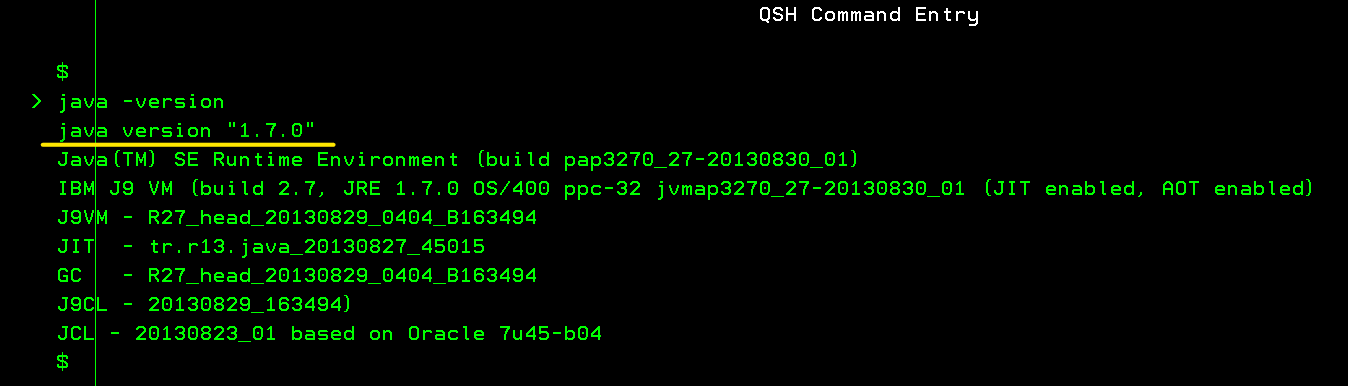
\includegraphics[width=0.7\textwidth]{img/java_version.png}
        \label{fig:java_version}
\end{figure}